\documentclass[letterpaper,10pt]{article}
\usepackage[utf8]{inputenc}
\usepackage[left=22mm,right=28mm,bottom=22mm,top=30mm]{geometry}
\usepackage[T1]{fontenc}
\usepackage[english]{babel}
\usepackage{color}
\usepackage[shadow,textwidth=22.8mm,color=roza,bordercolor=black,linecolor=roza]{todonotes}
\usepackage{soul}
\usepackage{fancyhdr}
\usepackage{graphicx}
\usepackage{amsmath}
\usepackage{mathtools}
\usepackage{fix-cm}
\usepackage[pdftex]{hyperref}
\usepackage{multirow}
\usepackage{colortbl}
\usepackage{array}
\usepackage{enumerate}
\usepackage{listings}
\usepackage{setspace}
\usepackage{tikz}
\usepackage{xcolor}
\usepackage[american]{circuitikz}
\usetikzlibrary{arrows,shapes,positioning}
\usetikzlibrary{circuits.logic.US}
\usetikzlibrary{calc} 
\usepackage{pgfplots}
\pgfplotsset{compat=1.14}
\usepackage{pgfkeys}
\usepackage{embedfile}
\hypersetup{
colorlinks,
citecolor=black,
filecolor=black,
linktoc=all,
linkcolor=black,
urlcolor=boja5,
}
\embedfile{logo.pdf}
\embedfile{Amp_Hf_A1_A2.tr}
\embedfile{Amp_Hf_A1_A5.tr}
\embedfile{Amp_Hf_A1_A9.tr}
\embedfile{Amp_Hf_A1_A15.tr}

\fancypagestyle{logo_stil}
{	\lhead{\small{\textsc{Haseljić Eldar}}} \chead{}	\rhead{\includegraphics[scale=0.05,trim={0.25mm 0.25mm 0.25mm 0.25mm},clip=true]{logo.pdf}}
	\lfoot{} \cfoot{\thepage} \rfoot{}
  	\renewcommand{\headrulewidth}{0.47pt}
  	\renewcommand{\footrulewidth}{0pt}
}

\newcounter{tabelica}
\setcounter{tabelica}{1}

\newcommand{\tabelica}[1]
{\vspace{4mm}
\stepcounter{tabelica}\hypertarget{tabelica:\arabic{tabelica}}{Tabelica}
\arabic{tabelica}: #1
\addcontentsline{lot}{table}{\arabic{tabelica}
\hspace{4mm} #1}
\vspace{4mm}}

\definecolor{roza}{RGB}{245,204,204}
\definecolor{boja1}{RGB}{194,42,20}
\definecolor{boja2}{RGB}{245,225,224}
\definecolor{boja3}{RGB}{0,255,0}
\definecolor{boja4}{RGB}{236,0,141}
\definecolor{boja5}{RGB}{0,173,238}
\definecolor{boja6}{RGB}{255,128,0}
\definecolor{boja7}{RGB}{238,31,155}
\definecolor{boja8}{RGB}{47,188,241}

\newcommand{\crveno}[1]
 {\textsl{\textbf{\color{boja1}#1\color{black}}}~}
\newcommand{\naredba}[1]
{\texttt{\color{boja1}\textbackslash{}#1\color{black}\{\}}}
\newcommand{\plavo}[1]
{\texttt{\color{blue}#1}\color{black}~}
\newcommand{\sretno}[1]
{\normalsize{\color{red}#1}\color{blue}~}

\definecolor{tikz1}{RGB}{236,236,168}
\definecolor{tikz2}{RGB}{245,211,221}
\definecolor{tikz3}{RGB}{197,220,173}
\definecolor{tikz4}{RGB}{141,153,224}
\definecolor{tikz5}{RGB}{208,209,203}
\definecolor{tikz6}{RGB}{156,67,65}
\definecolor{tikz7}{RGB}{118,108,151}
\definecolor{tikz8}{RGB}{239,239,181}
\definecolor{strijela}{RGB}{141,138,134}
\definecolor{znak}{RGB}{212,213,207}
\definecolor{tackica}{RGB}{185,189,193}
\definecolor{slova}{RGB}{77,77,95}

\begin{document}
\noindent{}\rmfamily{Univerzitet u Tuzli} \hfill{}	\textsc{Proljeće 2017} \\ 
\rmfamily{Fakultet elektrotehnike \hfill{}	Haseljić Eldar \\ Tehnologije za podršku tehničkom pisanju}
\vspace{6mm}
\begin{center}
\LARGE{}\textsc{Zadaća II iz Predmeta Tehnologije za Podršku
Tehničkom Pisanju}	\todo[]{\scriptsize{Naslov dokument
vertikalno je pomjeren za 6 mm u odnosu na prethodni i naredni sadržaj.}}
\vspace{6mm}

\renewcommand{\abstractname}{Abstract}
\begin{abstract}
\textbf{\textsl{U okviru zadaće II}} biti će demonstrirano svo stečeno znanje iz predmeta \textsl{Tehnologije za podršku tehničkom pisanju} vezano za \LaTeX. Studenti će \crveno{demonstrirati stečeno znanje}  na način da repliciraju sadržaj dokumenta (stranice od 1 do 6) pri čemu moraju obratiti pažnju na svaki detalj u originalnom dokumentu. Replicirani dokument mora biti \underline{vjerodostojna kopija} originalnom dokumentu (100\% kopija osim dijela prezime i ime, i broj indeksa). Kako rezultat, studenti će \textbf{\textsl{\color{blue}predati kod}} (*.tex file) prema pravilima definiranim na prethodnoj stranici teksta zadaće.
\end{abstract}
\end{center}

\renewcommand{\contentsname}{Kratak sadržaj}
\renewcommand{\listfigurename}{Kratka lista slika}
\renewcommand{\listtablename}{Kratka lista tabela}
\renewcommand{\figurename}{Sličica}
\renewcommand{\tablename}{Tabelica}
\tableofcontents
\listoffigures
\listoftables

\section{Stil dokumenta}
Redefiniranjem funkcionalnosti komande \naredba{contentsname} promijeniti naziv liste sadržaja u \textsl{Kratak sadržaj.} 
Na sličan način ponoviti za komande \naredba{listfigurename}, \naredba{listtablename}, \naredba{figurename} i \naredba{tablename} uslijed nedostatka podrške za govorno područje \textsl{Bosne i Hercegovine} u paketu \texttt{babel}.
\newpage
\pagestyle{logo_stil}
\subsection{Margine dokumenta}
Margine stranica dokumenta su postavljene na sljedeći način: lijeva i donja na 22 mm, desna na 28 mm i gornja na 30 mm. Na mjesto \textsl{Prezime Ime} upisat vaše \ul{prezime i ime}. \crveno{Obratiti pažnju} da se na tekućoj i narednim stranicama dokumenta zadaće, nalazi zaglavlje i podnožje a na prethodnoj ne! U okviru zadaće kreirati \LaTeX\ komande i okruženja samo na mjestima gdje to ima smisla.
\subsection{Zaglavlje i podnožje dokumenta}
\textrm{Stil dokumenta generirati sa komandama iz paketa \texttt{fancyhdr} pri čemu će se novi stil zvati \texttt{logo\_stil}. Slika unutar zaglavlja stranice dokumenta (\textsl{logo.pdf}), skalirana je na 0.05 a prostor oko slike skraćen je za 0.25 mm sa svih strana} \todo[]{\scriptsize{Upotrijebiti \texttt{trim} \& \texttt{clip} opcije}} . Debljina linije u zaglavlju je 0.47 pt.
\section{Matematički mod i tabele}
\subsection{Matematički mod}
Tokom semestra, u \LaTeX-u smo upoznali matematički mod\footnote{\crveno{Ne zaboravite} da matematički mod zahtjeva uključenje paketa \texttt{amsmath}.} koji nam omogućava i formatiranje matrica \\ \hfill{} 
\normalsize{\begin{equation*}
R_{xx}=x^T x = \begin{bmatrix}\begin{array}{ccc}
 x(-1) &  0 & 0 \\[2mm]
 x(0) & x(-1) & 0 \\[2mm]
 x(1) & x(0) & x(-1) \\[2mm]
 0 & x(1) & x(0)\\[2mm]
 0 & 0 & x(1)\\\end{array}
\end{bmatrix} = 
\begin{bmatrix}\begin{array}{ccc}
\dfrac{\alpha}{2} &  0 & 0 \\
 1 & \dfrac{\alpha}{2} & 0 \\
 \dfrac{\alpha}{2} & 1 & \dfrac{\alpha}{2} \\
 0 & \dfrac{\alpha}{2} & 1 \\
 0 & 0 & \dfrac{\alpha}{2} \\\end{array} 
\end{bmatrix} =
\begin{bmatrix}\begin{array}{ccc}
 1+\dfrac{\alpha^2}{2} &  \alpha & \dfrac{\alpha^2}{4} \\
 \alpha & 1+\dfrac{\alpha^2}{2} & \alpha \\
 \dfrac{\alpha^2}{4} & \alpha & 1+\dfrac{\alpha^2}{2} \\\end{array}
\end{bmatrix}
\end{equation*}} \\
\noindent{}U nastavku imamo primjer jedne \textsl{Bessel-ove} funkcije u integralnom obliku:\\ \hfill{}
\begin{equation}
I_\alpha (x)=\dfrac{1}{\pi}\int_{0}^{\pi} e^{x\cos(\theta)}  \cos  {(\alpha\theta)}~d\theta - \dfrac{\sin{(\alpha\pi)}}{\pi}  \int_{0}^{\infty} e^{-x\cosh(t)-\alpha t}dt
\end{equation}\\ \hfill{}
pri čemu se \textsl{Bessel-ove} funkcije $K_{1/3}$ i $K_{2/3}$ mogu izraziti kao:\\ \hfill{}
\normalsize{\begin{equation}
K_{\frac{1}{3}} (\epsilon)=~\sqrt[]{3} \int_{0}^{\infty} \exp \left[-\epsilon\left(1+\dfrac{4x^{2}}{3}\right)~\sqrt[]{1+\dfrac{x^{2}}{3}}\right]dx
\end{equation}}\hfill{}
\normalsize{\begin{equation}
K_{\frac{2}{3}} (\epsilon) = \dfrac{1}{\sqrt[]{3}}  \int_{0}^{\infty} \dfrac{3+2x^{2}}{\sqrt[]{1+\frac{x^{2}}{3}}} \exp\left[-\epsilon \left(1+\dfrac{4x^{2}}{3}\right)~\sqrt[]{1+\dfrac{x^{2}}{3}}\right]dx
\end{equation}}
\begin{flushleft}
\noindent{}U sljedećem redu upisati broj vašeg indeksa koristeći familiju fonta \textsl{New Century Schoolbook (pnc)} visine \textit{79 pt}\footnote{
Obratiti pažnju da će nam trebati paket \texttt{fix-cm}\vspace{18.5mm}}
\end{flushleft}\vspace{1mm}
\begin{center}
\fontsize{79pt}{6.5mm}\fontfamily{pnc}\selectfont{16116}
\end{center}
\newpage
\subsection{Tabele}
U nastavku imamo tri table postavljene koristeći okruženje \plavo{minipage}, \plavo{tabular}i \plavo{table}.\hfill{}
\begin{table}[h]
  \centering{}\small{}
\setstretch{1.1}
  \begin{tabular}{c c c}
  \hline \hline 
    \rowcolor[RGB]{77,77,77}\color {white}Put br. & \color{white}Redoslijed propagacije signala & \color {white}Težinski faktor $g_i$($f$)\\ \hline \hline
  \rowcolor[RGB]{242,242,242} 1 &  $A \rightarrow B \rightarrow C$ & $t_{1B}$ \\
  2 & $A \rightarrow B \rightarrow D \rightarrow B \rightarrow C$ & $t_{1B} r_{3D} t_{3B}$ \\
 \rowcolor[RGB]{242,242,242} \vdots & \vdots & \vdots  \\
  N & $A \rightarrow B (\rightarrow D \rightarrow B)^{N-1} \rightarrow C$ & $t_{1B}r_{3D}{(r_{3B}r_{3D})}^{N-2} t_{3B}$\\\hline \hline
  \end{tabular}
  
   \caption{Redoslijed propagacija signala u mreži}
 \label{Tabelica:tab1}
\end{table}\\[1mm] \hfill{}
\begin{minipage}[b]{0.5\textwidth}
  \centering{}\setstretch{1.3}
	\begin{tabular}{cc}
  \hline \hline  
  Bodovi & Ocjena \\ \hline 
  94 - 100 & 10 \\
  84 - 93 & 9 \\
  74 - 83 & 10\\
  64 - 73 & 9 \\
  54 - 63 & 10 \\ \hline \hline
  \end{tabular}
  
  \tabelica{Bodovi i ocjene}
\end{minipage}
\begin{minipage}[b]{0.5\textwidth}
\centering{}
\setstretch{1.3}  
\begin{tabular}{|l|c|r|}
  \hline \hline
	\cellcolor[RGB]{204,255,204}L1 & L2 & L3 \\ \hline 
 \multicolumn{2}{|c|}{\cellcolor[RGB]{204,204,255}MC1} & \multirow{2}{*}{MR1} \\ \cline{1-2} A & B & \\ \hline
  \multirow{2}{*}{MR2} &  \multicolumn{2}{c|}{MC2} \\ \cline{2-2} & D & \cellcolor[RGB]{255,230,204}E \\ \hline
  G & \cellcolor[RGB]{255,204,204}E & M  \\\hline \hline
  \end{tabular}
  
  \tabelica{Spajanje ćelija}
\end{minipage}\hfill{}
\begin{center}
\fbox{\colorbox{boja2}{\parbox{105mm}{U malom ograničenom paragrafu širine 105 mm prikazana je lista malih Grčkih karaktera, velikih rimskih cirata\footnote{} i heksadecimalnih cifara\footnote{}
\begin{enumerate}[a)]
\item \small{}$\alpha, ~\Delta, ~\sigma, ~\Gamma, ~\rho, ~\Psi, ~\mu, ~\gamma, ~\epsilon, ~\Omega, ~\psi, ~\pi, ~\kappa, ~\vartheta, ~\delta, ~\omega, ~\lambda, ~\tau.$ 
\item $I$, $V$, $X$, $L$, $D$, $C$ i $M$
\item \scriptsize{\texttt{0, 1, 2, 3, 4, 5, 6, 7, 8, 9, A, B, C, D, E i F}}
\end{enumerate}}}}
\end{center}

\noindent{}. \\
\noindent{}Sistem jednačina zapisanih prema \textit{Kirchhoff}-ovim zakonima, za neko elektirčno kolo je 
\begin{align}
i_1 - i_2 - i_3 & = 0 \\ \nonumber
-R_1 i_2 + \mathcal{E}_2 - R_2 i_1 &= 0 \\ \nonumber
-R_3 i_3 - \mathcal{E}_1 - \mathcal{E}_2 + R_1 i_2 &= 0 
\end{align}
\section{Paketi za crtanje u \LaTeX-u}
\subsection{TikZ paket}
Na slici \ref{Slicica:fig1}\footnote{Obavezno koristiti princip referenciranja sa komandom \naredba{ref}} prikazani su frekventni odzivi hipotetičkih sistema\footnote{Vrijednosti odziva sistema uključeni su u pdf-u teksta zadaće a legendu dijagrama dodati koristeći komaandu \naredba{addlegendentry}\vspace{4mm}} a u nastavku funkcije oblika $x(t) = \sin(180t)+0.4 \cdot rand$ i $y(t) = \sin(180t) \pm 0.5$ kreirane sa okruženjem \plavo{tikzpicture} i \plavo{axis}. Za crtanje konkretnih krivi koristiti komandu \naredba{addplot}. Aktiviranje mrežice na grafiku izvodimo sa opcijom \texttt{grid}. Postavke opsega grafika (\textit{plot-a}) su \texttt{xmin=-5,xmax=5,ymin=-4} i \texttt{ymax=4} u okviru \plavo{axis} okruženja. Za skaliranje dijagrama na slikama \ref{Slicica:fig2} i \ref{Slicica:fig3} koristiti opciju \texttt{scale} u okviru okruženja \plavo{tikzpicture}. 
\newpage
\begin{figure}
\centering{}
\begin{tikzpicture}[scale=1.1]
\begin{axis}[xlabel=$f(MHz)$,ylabel= $|H(f)|_{dB}$,xmin=0,xmax=50,ymax=20,grid=major,grid style={dotted},legend columns=4,legend style={font=\footnotesize{}}]
\addlegendentry{$\texttt{S1-S2}$}
\addlegendentry{$\texttt{S1-S5}$}
\addlegendentry{$\texttt{S1-S9}$}
\addlegendentry{$\texttt{S1-S15}$}
\addplot [blue, line width=0.8pt] table [x=f,y=H] {Amp_Hf_A1_A2.tr};\node at (40,-18){\footnotesize{\texttt{(S1-S2)}}};
\addplot[red,  line width=0.8pt] table [x=f,y=H] {Amp_Hf_A1_A5.tr};
\node at (40,-48){\footnotesize{\texttt{(S1-S5)}}};
\addplot[boja3,line width=0.8pt] table [x=f,y=H] {Amp_Hf_A1_A9.tr};
\node at (40,-82){\footnotesize{\texttt{(S1-S9)}}};
\addplot[boja4,line width=0.8pt] table [x=f,y=H] {Amp_Hf_A1_A15.tr};
\node at (40,-130){\footnotesize{\texttt{(S1-S15)}}};
\end{axis}

\end{tikzpicture}
\caption{Frekventni odzivi hipotetičkih sistema}
 \label{Slicica:fig1}
\end{figure}\vspace{1mm} \hfill{}
\begin{figure}
\begin{minipage}{0.5\textwidth}\centering{}
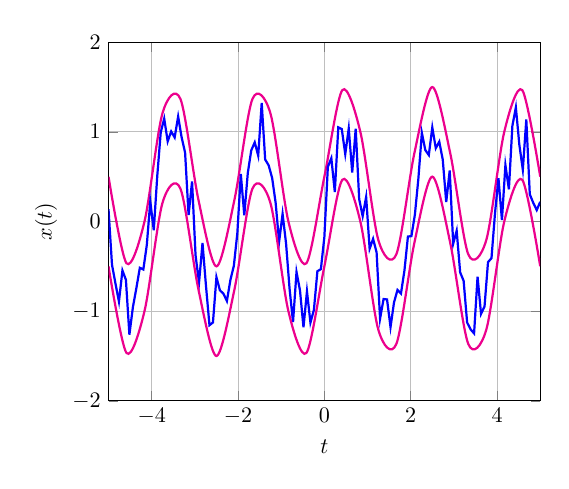
\begin{tikzpicture}[scale=0.8]
\begin{axis}[xlabel=$t$,ylabel=$x(t)$,xmin=-5,xmax=5,ymin=-2,ymax=2,grid=major,grid style={solid}]
\addplot[boja4,line width=1pt,smooth] expression{(sin(180*x))+0.5};
\addplot[domain=-5:5,blue,samples=125,line width=1pt] expression{sin(180*x)+0.4*rand};
\addplot[boja4,line width=1pt, smooth]expression{(sin(180*x))-0.5};
\end{axis}
\end{tikzpicture}
\caption{Sinusne funkcije sa i bez izobličenja}
 \label{Slicica:fig2}
\end{minipage}
\begin{minipage}{0.5\textwidth}\centering{}
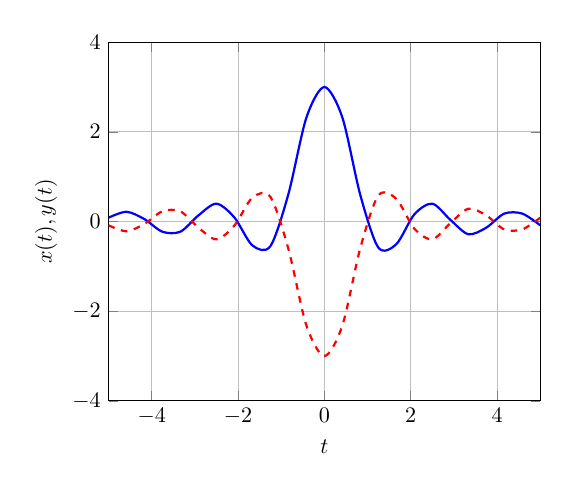
\begin{tikzpicture}[scale=0.8]
\begin{axis}[xlabel=$t$,ylabel=${x(t),y(t)}$,xmin=-5,xmax=5,ymin=-4,ymax=4,grid=major,grid style={solid}]
\addplot[blue,line width=1pt,smooth] expression{sin(180*x+x*x)/x};
\addplot[red,line width=1pt,dashed,smooth] expression{-sin(180*x+x*x)/x};
\end{axis}
\end{tikzpicture}
\caption{Verzije \texttt{sinc} funkcije}
 \label{Slicica:fig3}
\end{minipage}
\end{figure}\\\hfill{}
\noindent{}Na slici \ref{Slicica:fig3} prikazane su sljedeće funkcije:
\begin{align}
x(t)= \dfrac{\sin(180x+x^2)}{x} \\[1.5mm]
y(t)= -\dfrac{\sin(180x+x^2)}{x}
\end{align}
\vspace{6mm}
\subsection{Električne, blok sheme i \crveno{circuitikz} paket}
\noindent{}Na slici \ref{Slicica:fig4} prikazana je implementacija logičke funkcije\footnote{Prilikom crtanja logičke sheme neophodno je uključiti \textit{tikz} biblioteku \textit{circuits.logic.US}} $~f = AB + \overline{A}~\overline{B}~C$.  Ukoliko imate poteškoća\\ sa realizacijom logičke i električne sheme, možete se poslužiti primjerima iz kratkog \textit{manuala} \texttt{circutikz} paketa, koje se nalazi na CTAN \href{http://texdoc.net/texmf-dist/doc/latex/circuitikz/circuitikzmanual.pdf}{stranici}.\hfill{}
\newpage
\begin{figure}[h]
\centering{}
\begin{circuitikz}[circuit logic US,scale=0.95]
small{
\draw (0,0)node[above]{A}--(0,-8);
\draw (1,0)node[above]{B}--(1,-8);
\draw (2,0)node[above]{C}--(2,-8);}
\draw (3.5,-1.5)node[nand gate,logic gate inputs=nnn,scale=1.3](nikolo1){};
\draw (3.5,-4)node[nand gate,logic gate inputs=nn,scale=1.1](nikolo2){};
\draw (4,-5)node[nand gate,logic gate inputs=nn,scale=1.1](nikolo3){};
\draw (4,-6)node[nand gate,logic gate inputs=nn,scale=1.1](nikolo4){};
\draw (6.2,-5)node[nand gate,logic gate inputs=nnn,scale=1.3](nikolo5){};
\draw (6.2,-3)node[nand gate,logic gate inputs=nnn,scale=1.3](nikolo6){};
\draw (8.2,-2)node[nand gate,logic gate inputs=nnn,scale=1.4](nikolo7){};

\draw (0,-1.3)to[short,*-](nikolo1.input 1);
\draw (1,-1.5)to[short,*-](nikolo1.input 2);
\draw (2,-1.7)to[short,*-](nikolo1.input 3);
\draw (nikolo1.output)--(5,-1.5)|-(nikolo7.input 1);
\draw (2,-4)to[short,*-*](2.5,-4)|-(nikolo2.input 1);
\draw (2.5,-4)|-(nikolo2.input 2);
\draw (nikolo2.output)--(4.5,-4)|-(nikolo6.input 3);
\draw (0,-5)to[short,*-*](3,-5)|-(nikolo3.input 1);
\draw (3,-5)|-(nikolo3.input 2);
\draw (nikolo3.output)--(5,-5)|-(nikolo5.input 1);
\draw (1,-6)to[short,*-*](3,-6)|-(nikolo4.input 1);
\draw (3,-6)|-(nikolo4.input 2);
\draw (nikolo4.output)--(5.2,-6)|-(nikolo5.input 2);
\draw (2,-7)to[short,*-](5.5,-7)|-(nikolo5.input 3);
\draw (nikolo5.output)--(7.5,-5)|-(nikolo7.input 3);
\draw (0,-2.8)to[short,*-](nikolo6.input 1);
\draw (1,-3) to[short,*-](nikolo6.input 2);
\draw (nikolo6.output)--(7.2,-3)|-(nikolo7.input 2);
\draw (nikolo7.output)--(9.7,-2)node[above]{$f$};
\end{circuitikz}


\caption{Implementacija logičke funkcije $f$ sa NAND logičkim kolima}
 \label{Slicica:fig4}
\end{figure}\hfill{}

\noindent{}Na slici \ref{Slicica:fig5} prikazana je ekvivalentna shema jednog hipotetičkog pojčavačkog stepena. \todo{\scriptsize{}Upotrijebiti opciju \texttt{american}
u okruženju \plavo{circuitikz} za generiranje simbola prema američkom standardu označavanja elektroničkih komponenti.} U okviru električne sheme (na slici \ref{Slicica:fig5}) korištene su ljedeće komponente: \texttt{R}, \texttt{L,C} i \texttt{american current source.}\\
\begin{figure}[h]
\centering{}
\begin{circuitikz}[circuit logic US,american,scale=0.9]
\normalsize{}
\draw (0,0) node[ocirc]{};
\draw (0,-0.7) node[above]{$+$};
\draw (0,-1.5) node{$u_{ul}$};
\draw (0,-2.2) node[below]{$-$};
\draw[->,>=latex',rounded corners=5pt,line width=1pt,color=red](0.5,-1.5)--(0.5,-0.5)--(4,-0.5)--(4,-2.5)--(0.5,-2.5);

\draw (0,0) to[short,i_=$i_{ul}$](2,0) node[above]{$A_1$};
\draw (2,0) to[R, l_=$R_1$,*-*, i=$i_2$] (5,0) node[above]{$B_1$};
\draw (8,0) to[I,l=$gi_1$,color=boja6] (5,0);
\draw (8,0) --(9,0)node[above]{$D_1$};
\draw (9,0) to[R,l_=$R_C$, i=$i_C$] (12,0) node[above]{$E_1$};
\draw (12,0) to[short,*-] (14,0);
\draw (14,0) to[short,i_=$i_{iz}$] (15.5,0);
\scriptsize{
\draw (9.2,-0.7) node[above]{$+$};
\draw (9.2,-1.5) node{$u_{12}$};
\draw (9.2,-2.2) node[below]{$-$};}

\draw[->,rounded corners=5pt,line width=1pt,color=blue,dashed](9.5,-1.5)--(9.5,-0.5)--(14.5,-0.5)--(14.5,-2.5)--(9.5,-2.5);

\draw (0,-3) node[ocirc]{};
\draw (0,-3) to[short,-*] (2,-3) to[short,-*] (5,-3) to[short,-*] (11,-3) -- (15.5,-3);

\draw [color=black](2,-6) to[L, l^=$L_2$,i=$i_5$,color=boja7] (5,-6);
\draw (5,-6) to[R=$R_6$, i=$i_6$] (8,-6) -- (11,-6) to[,short,-*] (11,-3);

\draw (2,0) to[C=$C_1$, i=$i_1$,] (2,-3) to[C=$C_3$, i=$i_5$] (2,-6);
\draw (5,0) to[C,l_=$C_{E1}$, i=$i_{e1}$] (5,-3) to[R=$R_5$, i=$i_6$,] (5,-6);
\draw [color=black](8.5,0) to[L,l_=$L_1$,color=boja7,*-*, i=$i_4$](8.5,-3) ;
\draw (12,-3)node[below]{$F_1$} to[I, l=$hi_2$,color=boja6] (12,0) ;
\draw (14,0) to[R, l_=$Z_{E2}$] (14,-3);
\draw [color=black](15.5,0) to[R, l_=$R_p$,color=boja8] (15.5,-3);

\draw (16.2,-0.7) node[above]{$+$};
\draw (16.2,-1.5) node{$u_{iz}$};
\draw (16.2,-2.2) node[below]{$-$};

\end{circuitikz}
\caption{Ekvivalentna shema hipotetičkog pojačavača}
 \label{Slicica:fig5}
\end{figure}\\
\noindent{}Slika \ref{Slicica:fig6} predstavlja model jednog komunikacijskog sistema. Prilikom crtanja modela i ostalih \texttt{tikz} baziranih dijagrama/grafika/slika možete se poslužiti aplikacijama kao što je \textsl{ktikz, QTikZ, TpX,fredokun TikZ-Editor} i sl.\\
\newpage
\begin{figure}[h]
\centering{}
\tikzstyle{blok1} = [draw=gray,shading=axis,rectangle,right color=tikz1,left color=tikz1!30!white,shading angle=30,line width=1pt,minimum width=25mm,minimum height = 10mm,rounded corners=2pt,drop shadow]
\tikzstyle{blok2} = [shading=axis,rectangle,right color=tikz2,left color=white!30!white,shading angle=60,minimum width=20mm,minimum height = 10mm,rounded corners=2pt,line width=1pt,draw=gray,drop shadow]
\tikzstyle{blok3} = [shading=axis,rectangle,right color=tikz3,left color=tikz3!15!white,shading angle=30,line width=1pt,draw=gray,minimum width=20mm,minimum height = 10mm,rounded corners=2pt,drop shadow]
\tikzstyle{blok4} = [draw=gray,rectangle,right color=tikz4,left color=tikz4!30!white,shading angle=30,line width=1pt,draw=gray,minimum width=20mm,minimum height = 10mm,rounded corners=2pt,drop shadow]
\tikzstyle{blok5} = [shading=axis,rectangle,right color=tikz5,left color=white!30!white,shading angle=60,line width=1pt,draw=gray,minimum width=18mm,minimum height = 8mm,rounded corners=2pt,drop shadow]
\tikzstyle{blok6} = [rectangle,right color=tikz6,left color=tikz6!30!white,shading angle=30,line width=1pt,draw=gray,minimum width=20mm,minimum height = 10mm,rounded corners=2pt,drop shadow]
\tikzstyle{blok7} = [rectangle,right color=tikz7,left color=tikz7!30!white,shading angle=30,line width=1pt,draw=gray,minimum width=20mm,minimum height = 10mm,rounded corners=2pt,drop shadow]
\tikzstyle{blok8} = [draw=gray,rectangle,right color=tikz8,left color=tikz8!30!white,shading angle=60,line width=1pt,draw=gray,minimum width=20mm,minimum height = 10mm,rounded corners=2pt,drop shadow]
\tikzstyle{znak} = [draw, circle,minimum size=1pt,right color=znak,left color=white!5!,shading angle=30,line width=1pt,draw=gray,drop shadow,scale=0.8]
\tikzstyle{tackica} = [fill, circle,minimum size=1pt, right color=tackica,left color=white!5!,shading angle=30,line width=1pt,draw=gray,scale=0.5]
\tikzstyle{input} = [coordinate]
\begin{tikzpicture}[scale=0.5]
\textbf{
\draw (-9.5,8)node[blok1](A1){$ $};
\draw (A1) node[yshift=2.5mm]{\color{slova}\textsf{\scriptsize{SLUČAJNI}}};
\draw (A1) node[yshift=0mm]{\color{slova}\textsf{\scriptsize{GENERATOR}}};
\draw (A1) node[yshift=-2.5mm]{\color{slova}\textsf{\scriptsize{BINARNOG TOKA}}};
\draw (-2,8)node[blok2](A2){$ $};
\draw (A2) node[yshift=0mm]{\color{slova}\textsf{\scriptsize{QAM MAPER}}};
\draw (5.,8)node[blok3](A3){$ $};
\draw (A3) node[yshift=2.5mm]{\color{slova}\textsf{\scriptsize{SQRT}}};
\draw (A3) node[yshift=0mm]{\color{slova}\textsf{\scriptsize{PODIGNUTI}}};
\draw (A3) node[yshift=-2.5mm]{\color{slova}\textsf{\scriptsize{KOSINUS}}};
\draw (11,8)node[blok5](A4){$ $};
\draw (A4) node[yshift=0mm]{\color{slova}\textsf{\scriptsize{KANAL}}};
\draw (8,12)node[blok4](A5){$ $};
\draw (A5) node[yshift=2mm]{\color{white}\textsf{\scriptsize{DIJAGRAM}}};
\draw (A5) node[yshift=-1.5mm]{\color{white}\textsf{\scriptsize{OKA}}};
\draw (18,12)node[blok6](A6){$ $};
\draw (A6) node[yshift=0mm]{\color{white}\textsf{\small{AWGN}}};
\draw (18,8)node[znak](znak){$\mathbf{+}$};
\draw (-6,2)node[blok8](A7){$ $};
\draw (A7) node[yshift=0mm]{\color{slova}\textsf{\small{BER}}};
\draw (-6,-2)node[blok2](A8){$ $};
\draw (A8) node[yshift=0mm]{\color{slova}\textsf{\scriptsize{QAM DEMAPER}}};
\draw (5.5,-2)node[blok3](A9){$ $};
\draw (A9) node[yshift=2mm]{\color{slova}\textsf{\scriptsize{OPTIMALNI}}};
\draw (A9) node[yshift=-1.5mm]{\color{slova}\textsf{\scriptsize{DETEKTOR}}};
\draw (11.5,-2)node[blok7](A10){$ $};
\draw (A10) node[yshift=0mm]{\color{white}\textsf{\scriptsize{EKVALIZATOR}}};
\draw (18,-2)node[blok3](A11){$ $};
\draw (A11) node[yshift=2mm]{\color{slova}\textsf{\scriptsize{OPTIMALNI}}};
\draw (A11) node[yshift=-1.5mm]{\color{slova}\textsf{\scriptsize{FILTER}}};
\draw (1.5,4)node[blok4](A12){$ $};
\draw (A12) node[yshift=2mm]{\color{white}\textsf{\scriptsize{SCATTER}}};
\draw (A12) node[yshift=-1.5mm]{\color{white}\textsf{\scriptsize{PLOT}}};}

\draw[->,>=latex',solid,color=strijela,line width=1.5pt] (A1) -- (A2);
\draw[->,>=latex',solid,color=strijela,line width=1.5pt] (A2) -- (A3);
\draw[->,>=latex',solid,color=strijela,line width=1.5pt] (A3) -- (A4);
\draw[->,>=latex',solid,color=strijela,line width=1.5pt] (A4) -- (znak);
\draw[->,>=latex',solid,color=strijela,line width=1.5pt] (znak) -- (A11);
\draw (-6,8)node[tackica](T1){};
\draw (1.5,8)node[tackica](T2){};
\draw (8,8) node[tackica](T3){} ;
\draw (14,8) node[tackica](T4){};
\draw[->,>=latex',solid,color=strijela,line width=1.5pt] (T1) -- (A7);
\draw[->,>=latex',solid,color=strijela,line width=1.5pt] (T3) -- (A5);
\draw[->,>=latex',solid,color=strijela,line width=1.5pt] (A8) -- (A7);
\draw[->,>=latex',solid,color=strijela,line width=1.5pt] (A9) -- (A8);
\draw (1.5,-2) node[tackica](T5){};
\draw[->,>=latex',solid,color=strijela,line width=1.5pt] (T5) -- (A12);
\draw[->,>=latex',solid,color=strijela,line width=1.5pt] (T2) -- (A12);
\draw[->,>=latex',solid,color=strijela,line width=1.5pt] (A6) -- (znak);
\draw[->,>=latex',solid,color=strijela,line width=1.5pt] (A11) -- (A10);
\draw[->,>=latex',solid,color=strijela,line width=1.5pt] (A10) -- (A9);
\draw[solid,color=strijela,line width=1.5pt] (T4) -- (14,12);
\draw[->,>=latex',solid,color=strijela,line width=1.5pt] (14.05,12) -- (A5);
\draw[solid,color=strijela,line width=1.5pt] (T4) -- (14,4);
\draw[->,>=latex',solid,color=strijela,line width=1.5pt] (14.05,4) -- (A12);
 
\end{tikzpicture}
\caption{Primjer modela komunikacijskog sistema} \label{Slicica:fig6}
\end{figure}\hfill{}
\begin{flushright}
\vfill{}
\sretno{Sretno} kodiranje!
\end{flushright}

\end{document}
